\section{Experimental setup}

\begin{figure}[htb]
  \begin{minipage}{0.49\hsize}
    \centering
    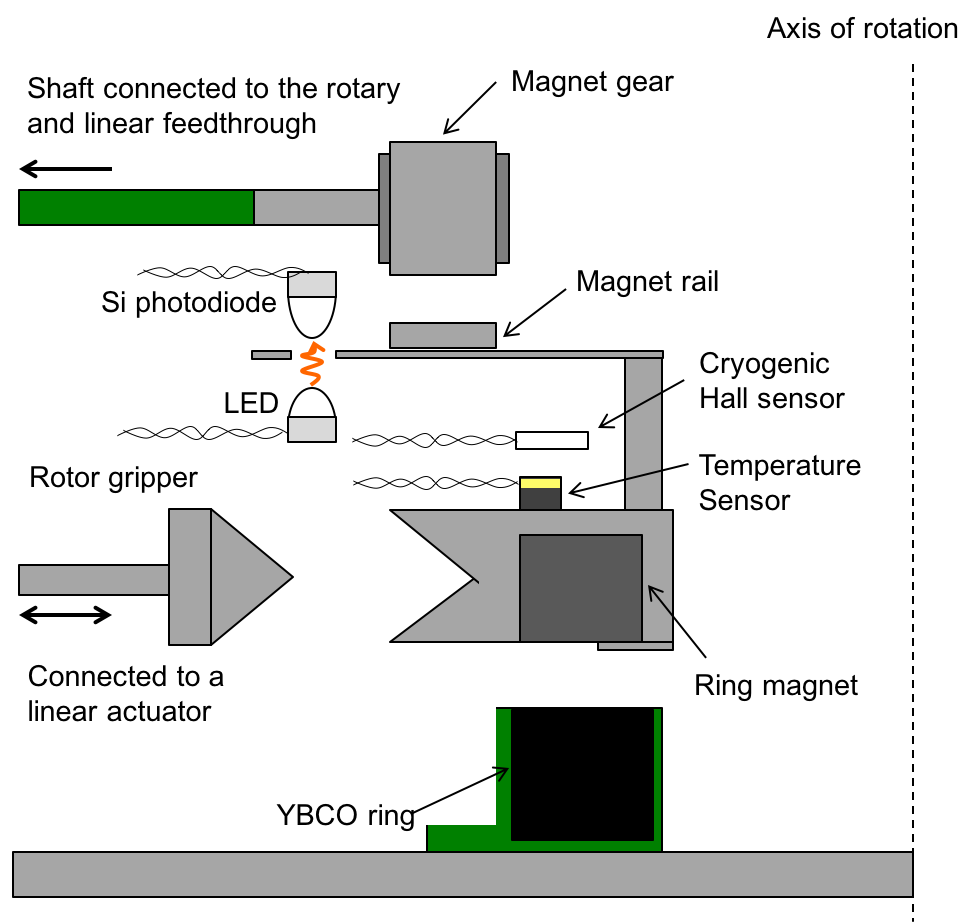
\includegraphics[width=65mm]{../figs/XsecView.eps}%
  \end{minipage}
  \begin{minipage}{0.49\hsize}
    \centering
    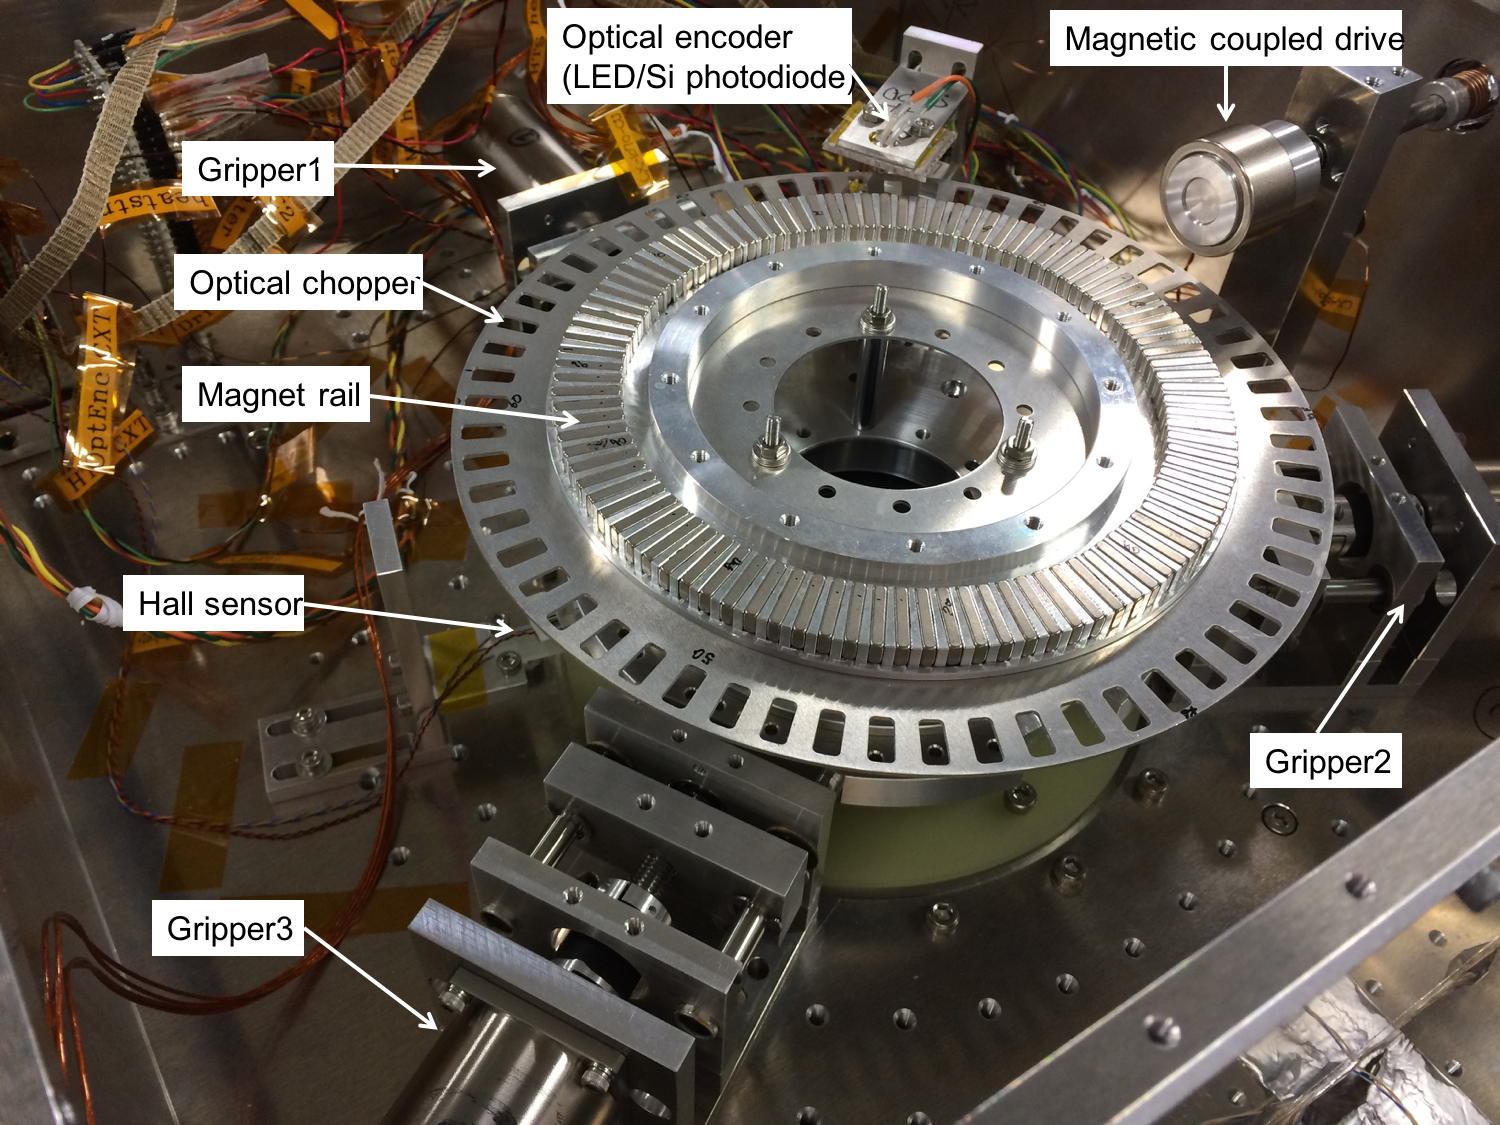
\includegraphics[width=65mm]{../figs/PhotoView.eps}%
  \end{minipage}
  \caption{The cross-sectional view and overview of experimental setup.}
  \label{fig:ExpSetup}
\end{figure}

Fig. \ref{fig:ExpSetup} shows cross section view of SMB experimental setup,
which is mainly constructed with a rotor, a stator and a rotor holding system.
The rotor is a NdFeB Permanent Magnet ring (PM) with 1.1 Tesla remnants, inserted into aluminum frame.
The stator is a YBCO superconductor ring type array with critical temperature of more than 90~K,
refrred to as a High Temperature Superconducting (HTS).
As the holding system, three holder arms with cryogenic stepping motors are mounted
to hold the rotor in place above the critical temperature of the HTS.

A cryogenic hall sensor is mounted above the PM to measure rotor magnetic field.
The hall sensor output is used as a levitation monitor, and also used as an encoder by magnetic field non-uniformity in roration.

A resistance temperature sensor is partly mounted on the PM by a screw
in order to measure the dependence between the hall sensor output and actual temperature.
Therefore, a contanious roration is not allowed when the temperature sensor is mounted.


\begin{itemize}
\item inside including the SMB
\item hall sensor and temperature sensor
\item temperature sensor accuracy
\item DAQ
\end{itemize}
